\documentclass{article}
\usepackage{graphicx}
\usepackage{blindtext}
\usepackage{titlesec}
\usepackage{subfig}
\usepackage{kinematikz}
\usepackage{ragged2e}
\usepackage{amsmath}
\usepackage{caption}
\usepackage{slashbox}
\usepackage[hidelinks]{hyperref}
\usepackage{float}
\usepackage[super]{nth}
\usepackage[bottom]{footmisc}
\usepackage{matlab-prettifier}
\usepackage[backend=biber]{biblatex}
\usetikzlibrary{calc,patterns,angles,quotes}

\title{
    Master's degree in Computer Engineering for Robotics and Smart Industry \\
    \vspace{0.5cm}
    Advanced control systems \\
    \vspace{0.5cm}
    \large Course assignments
}
\author{Enrico Bonoldi - VR502852}
\date{February 2025}

\begin{document}


\maketitle
\newpage
\tableofcontents
\newpage


\section{Introduction}

This techical report is about the assignments of the \textbf{Advanced control systems} course.
\\
The code is available at \hyperlink{https://github.com/bonoldie/ACS}{Github}.

\section{Robot structure and kinematics}
\label{sec:kinematics}

\begin{figure}[!h]
    \centering
    \subfloat{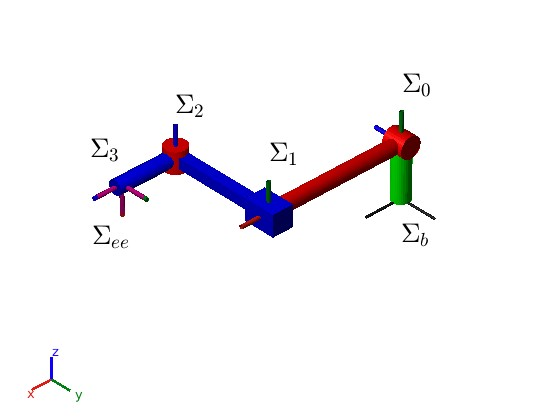
\includegraphics[width=0.5\linewidth]{robot/robot_home_conf.jpg}}
    \hfill
    \subfloat{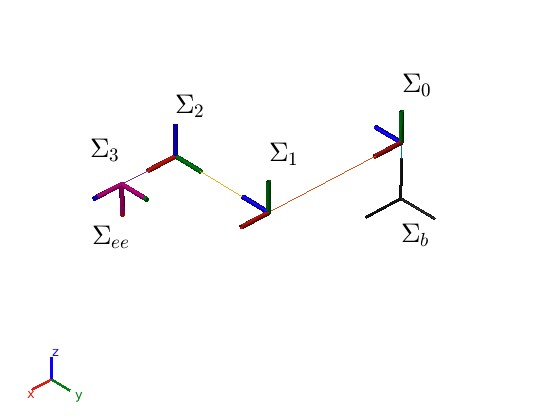
\includegraphics[width=0.5\linewidth]{robot/robot_home_conf_no_link.jpg}}
    \caption{Robot visualization}
    \label{fig:robot-visualization}
\end{figure}

\begin{align}
    \delta_{b-0} & = 0.15 \label{eq:delta_b_0} \\
    \delta_{0-1} & = 0.4 \label{eq:delta_0_1}  \\
    \delta_{1-2} & = 0.3 \label{eq:delta_1_2}  \\
    \delta_{2-3} & = 0.16 \label{eq:delta_2_3}
\end{align}

\subsection{DH table}

\setlength{\tabcolsep}{10pt} % Default value: 6pt
\renewcommand{\arraystretch}{1.8}
\begin{center}
    \begin{tabular}{ |c|c|c|c| }
        \hline
        a              & $\alpha$         & d                    & $\theta$ \\
        \hline
        0              & $\frac{\pi}{2}$  & $\delta_{b-0}$       & 0        \\
        $\delta_{0-1}$ & 0                & 0                    & $q_1$    \\
        0              & $-\frac{\pi}{2}$ & $\delta_{1-2} + q_2$ & 0        \\
        $\delta_{2-3}$ & 0                & 0                    & $q_3$    \\
        \hline
    \end{tabular}
\end{center}

To have the same alignment at the end-effector as the one in from the robotic toolbox we must rotate around the y axis (of the frame $\sigma_3$) by $\frac{\pi}{2}$ rad.

\subsection{Direct kinematics}



\begin{equation}
    T_{i}^{i-1} = \begin{bmatrix}
        \cos(\theta) & -\sin(\theta)\cos(\alpha) & \sin(\theta)\sin(\alpha)  & a\cos(\theta) \\
        \sin(\theta) & \cos(\theta)\cos(\alpha)  & -\cos(\theta)\sin(\alpha) & a\sin(\theta) \\
        0            & \sin(\alpha)              & \cos(\alpha)              & d             \\
        0            & 0                         & 0                         & 1
    \end{bmatrix}
    \label{eq:homogenous_transformation_mat}
\end{equation}

\subsection{Inverse kinematics}
A closed for solution of the inverse kinematics problem can be found by considering only the cartesian coordinates of the end-effector (since we have only 3 DoF).

\begin{flalign}
     & x_{ee} = 0.4\,\cos(q_1) + 0.16\,\cos(q_1)\cos(q_3) \label{eq:x_ee}        \\
     & y_{ee} = 0.16\,\sin(q_3) - q_2 - 0.3 \label{eq:y_ee}                      \\
     & z_{ee} = 0.4\,\sin(q_1) + 0.16\,\cos(q_3)\sin(q_1) + 0.15 \label{eq:z_ee}
\end{flalign}

TODO: calculations?

\begin{flalign}
     & q_1 = \arctan\left({\frac{z_{ee} - 0.15}{x_{ee}}}\right) \label{eq:q_1}                         \\
     & q_3 = \arccos\left(\frac{z_{ee} - 0.15 - 0.4\,\sin{q_1}}{0.16\,\sin(q_1)}\right) \label{eq:q_3} \\
     & q_2 = 0.16\,\sin\left(q_3\right) - 0.3 - y_{ee}\label{eq:q_2}
\end{flalign}
\\
Figure(\ref{fig:ik}) shows the case in which multiple valid solutions exists.

\begin{figure}
    \centering
    \subfloat[][Robotics system toolbox]{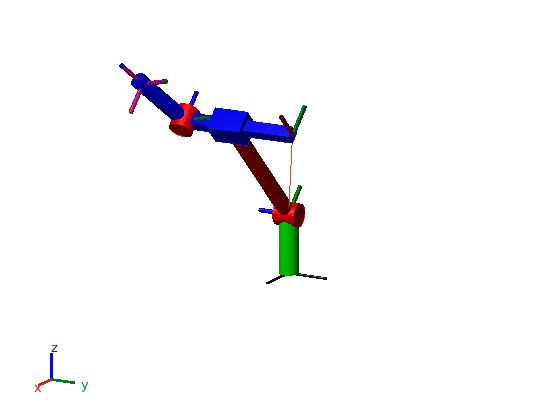
\includegraphics[width=0.5\linewidth]{robot/toolbox_ik.jpg}}
    \hfill
    \subfloat[][Inverse kinematics using equations (\ref{eq:q_1})(\ref{eq:q_3})(\ref{eq:q_2})]{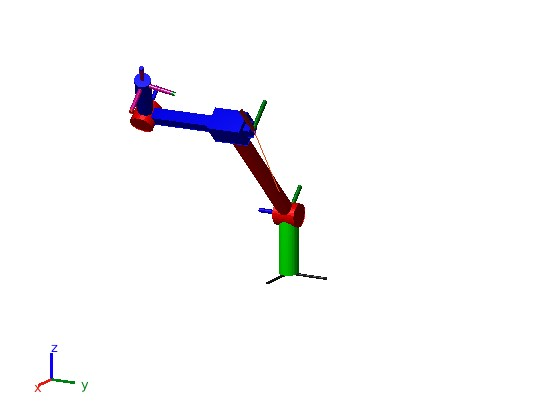
\includegraphics[width=0.5\linewidth]{robot/my_ik.jpg}}
    \caption{Inverse kinematics solutions}
    \label{fig:ik}
\end{figure}

\subsection{Jacobian matrices}

The Euler angles sequence chosen for the analytical Jacobian matrix is \textbf{\textit{ZYZ}}.


\section{Manipulator dynamics}
\subsection{Potential energy}

\begin{flalign}
    \mathcal{U}(q) = g\sin\left(q_1\right) + 0.7848\cos\left(q_3\right)\sin\left(q_1\right) + 4.4145
    \label{eq:potential_energy}
\end{flalign}

Where g is the gravitational acceleration.

\subsection{Kinetic energy}

\begin{equation}
    \begin{aligned}
        %    \mathcal{T}(q,\dot{q}) &= \dot{q_3}(0.0128\,\dot{q_3} - 0.04\,\dot{q_2}\cos(q_3)) \\ 
        %        & +  0.5\,\dot{q_1}^2(0.0640\,\cos(q_3) + 0.0126\,\cos(q_3)^2 + 0.4105)         \\ 
        %        & + \dot{q_2}(\dot{q_2} -  0.04\,\dot{q_3}\cos(q_3))
        \mathcal{T}(q,\dot{q}) & = 0.0063\,\dot{q_1}^2\,\cos\left(q_3\right)^2+0.0320\,\dot{q_1}^2\,\cos\left(q_3\right)+0.2653\,\dot{q_1}^2+\dot{q_2}^2 \\
                               & \quad-0.0800\,\dot{q_2}\,\dot{q_3}\,\cos\left(q_3\right)+0.0128\,\dot{q_3}^2
    \end{aligned}
    \label{eq:kinetic_energy}
\end{equation}

\subsection{Dynamic model}

\begin{equation}
    B(q) = \begin{bmatrix}
        0.064\,\cos(q_3) + 0.0126\,\cos(q_3)^2 + 0.5305 & 0               & 0               \\
        0                                               & 2               & -0.08\,cos(q_3) \\
        0                                               & -0.08\,cos(q_3) & 0.0256
    \end{bmatrix}
    \label{eq:dynamics_B}
\end{equation}


\begin{equation}
    C(q, \dot{q}) = \begin{bmatrix}
        -\dot{q_3}\,(0.0063\,\sin(2\,q_3)) + 0.032\,\sin(q_3) & 0 & -\dot{q_1}\,(0.0063\,\sin(2\,q_3) + 0.032\,\sin(q_3)) \\
        0                                                     & 0 & 0.08\,\dot{q_3}\,\sin(q_3)                            \\
        \dot{q_1}\,(0.0063\,\sin(2\,q_3) + 0.032\,\sin(q_3))  & 0 & 0
    \end{bmatrix}
    \label{eq:dynamics_C}
\end{equation}


\begin{equation}
    g(q) = \begin{bmatrix}
        0.3924\,\cos(q_1)\,(2\,\cos(q_3) + 25) \\
        0                                      \\
        -0.7848\,\sin(q_1)\,\sin(q_3)          \\
    \end{bmatrix}
    \label{eq:dynamics_G}
\end{equation}

\begin{equation}
    B(q)\,\ddot{q} + C(q, \dot{q})\,\dot{q} + g(q) = \tau \\
    \label{eq:eq_motion}
\end{equation}

Equation(\ref{eq:eq_motion}) is a set of 3 nonlinear second-order differential equations.

\iffalse
    TODO: this one is close but wrong!
    \begin{equation}
        \begin{bmatrix}
            0.3924\,\cos(q1)\,(2\,\cos(q3) + 25) + \ddot{q_1}\,(0.0640\,\cos(q3)              \\
            + 0.0126\,\cos(q3)^2 + 0.4105) - 2\,\dot{q_1}\,\dot{q_3}\,(0.0320\,\sin(q3)       \\
            + 0.0126\,\cos(q3)\,\sin(q3))                                                     \\
            \\
            0.0800\,\sin(q3)\,\dot{q_3}^2 + 2\,\ddot{q_2} - 0.0800\,\ddot{q_3}\,\cos(q3)      \\
            \\
            (0.0320\,\sin(q3) + 0.0126\,\cos(q3)\,\sin(q3))\,\dot{q_1}^2 + 0.0256\,\ddot{q_3} \\
            - 0.7848\,\sin(q1)\,\sin(q3) - 0.0800\,\ddot{q_2}\,\cos(q3)
        \end{bmatrix} = \begin{bmatrix}
            \tau_1 \\
            \tau_2 \\
            \tau_3
        \end{bmatrix}
        \label{eq:eq_motion_explicit}
    \end{equation}
\fi

\subsection{RNE formulation}
Using the Newton–Euler equations it is possible to set up an algorithm composed by a \textbf{forward recursion} step in which we propagate the links velocity and acceleration from the base link to the EE and a \textbf{backward recursion} step in which we propagate the forces from the EE to the base link.

TODO: add B,C*qdot,g matrices from the newton-euler approach

\subsection{Dynamic model in the operational space}

TODO: add just matrices T and J or all of them? ask the others

\subsection{Bonus: Parameters estimation}

\noindent
\begin{figure}[H]
    \captionsetup{justification=centering}
    \noindent\makebox[\textwidth]{
        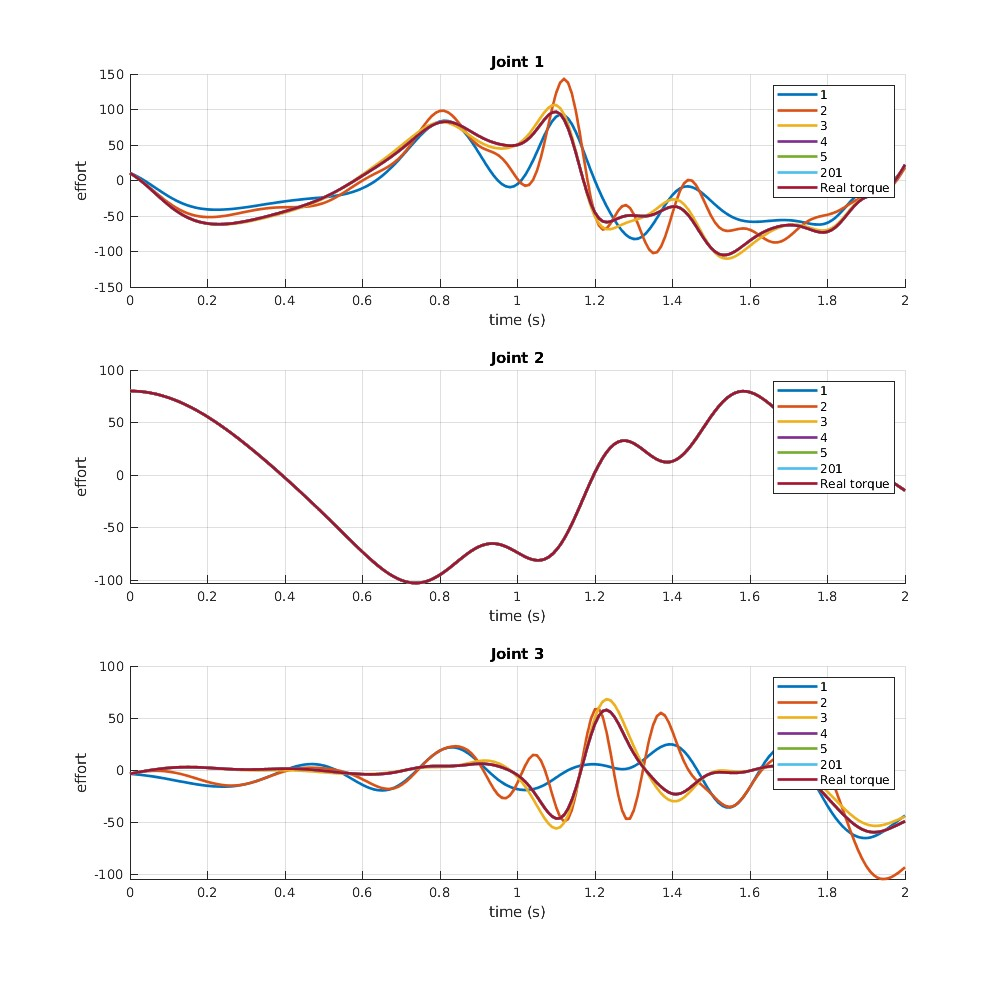
\includegraphics[scale=0.5]{param_estim/param_estim.jpg}
    }
    \caption{Parameters estimation \\ different simulation steps amount are taken into account}
    \label{fig:param_estim}
\end{figure}

\noindent
\begin{figure}[H]
    \captionsetup{justification=centering}
    \noindent\makebox[\textwidth]{
        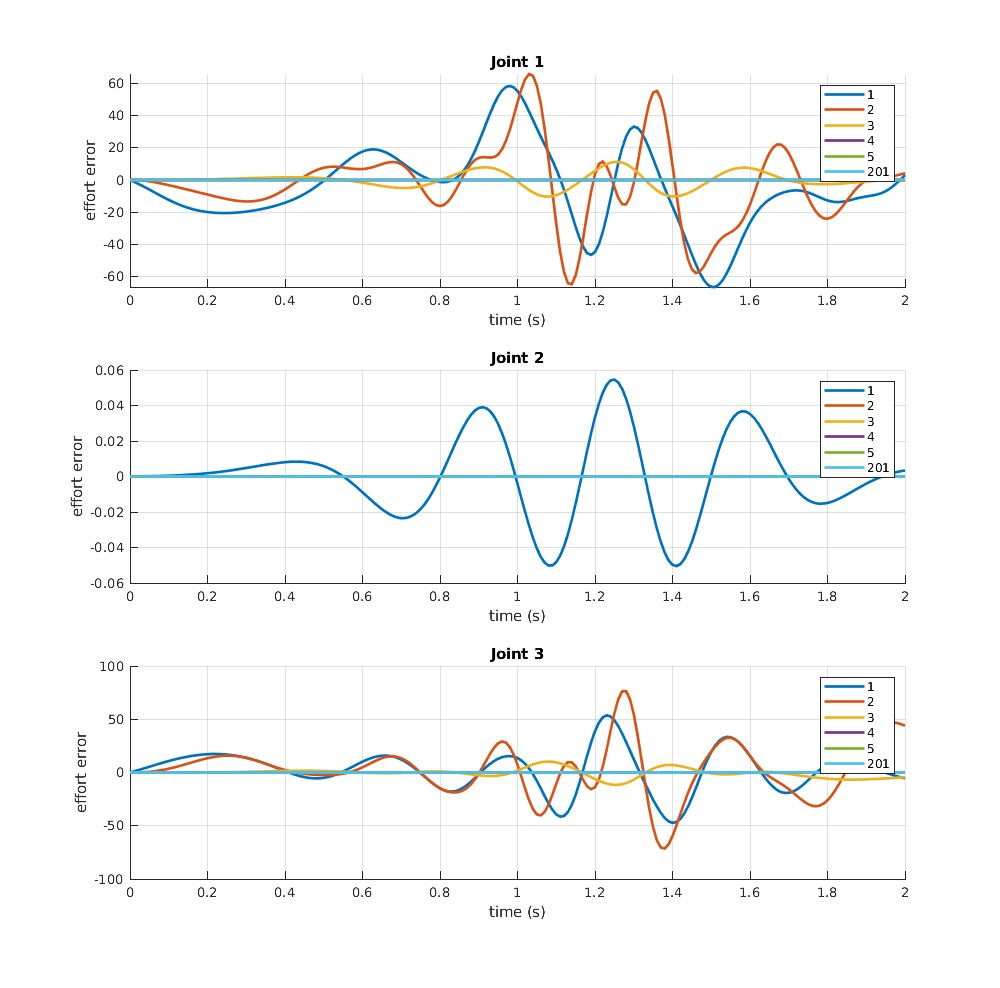
\includegraphics[scale=0.5]{param_estim/param_estim_error.jpg}
    }
    \caption{Parameters estimation error \\ different simulation steps amount are taken into account}
    \label{fig:param_estim_error}
\end{figure}



\begin{table}
    \begin{tabular}{|c|c|c|}
        \hline
        \backslashbox{Link \#}{Property} & Mass & Inertia tensor (w.r.t. CoM) \\
        \hline
        1                                & 1    & $\begin{bmatrix}
                                                           0.0002 & 0      & 0      \\
                                                           0      & 0.0800 & 0      \\
                                                           0      & 0      & 0.0800
                                                       \end{bmatrix}$   \\
        2                                & 1    & $\begin{bmatrix}
                                                           0.0076 & 0      & 0      \\
                                                           0      & 0.0150 & 0      \\
                                                           0      & 0      & 0.0076
                                                       \end{bmatrix}$   \\
        3                                & 1    & $\begin{bmatrix}
                                                           0.0002 & 0      & 0      \\
                                                           0      & 0.0128 & 0      \\
                                                           0      & 0      & 0.0128
                                                       \end{bmatrix}$   \\
        \hline
    \end{tabular}
    \caption{Real robot parameters}
    \label{tab:real_params}
\end{table}

\begin{table}
    \begin{tabular}{|c|c|c|}
        \hline
        \backslashbox{Link \#}{Property} & Mass & Inertia tensor (w.r.t. CoM) \\
        \hline
        1                                & 1    & $\begin{bmatrix}
                                                           0 & 0 & 0      \\
                                                           0 & 0 & 0      \\
                                                           0 & 0 & 0.0406
                                                       \end{bmatrix}$             \\
        2                                & 1    & $\begin{bmatrix}
                                                           0 & 0      & 0 \\
                                                           0 & 0.0406 & 0 \\
                                                           0 & 0      & 0
                                                       \end{bmatrix}$             \\
        3                                & 1    & $\begin{bmatrix}
                                                           0.0140 & 0      & 0      \\
                                                           0      & 0.0266 & 0      \\
                                                           0      & 0      & 0.0128
                                                       \end{bmatrix}$   \\

        \hline
    \end{tabular}
    \caption{Estimated robot parameters}
    \label{tab:estimated_params}
\end{table}

\section{Control schemes}

\subsection{Joint Space PD control law with gravity compensation}

\begin{figure}[H]
    \noindent
    \makebox[\textwidth]{
        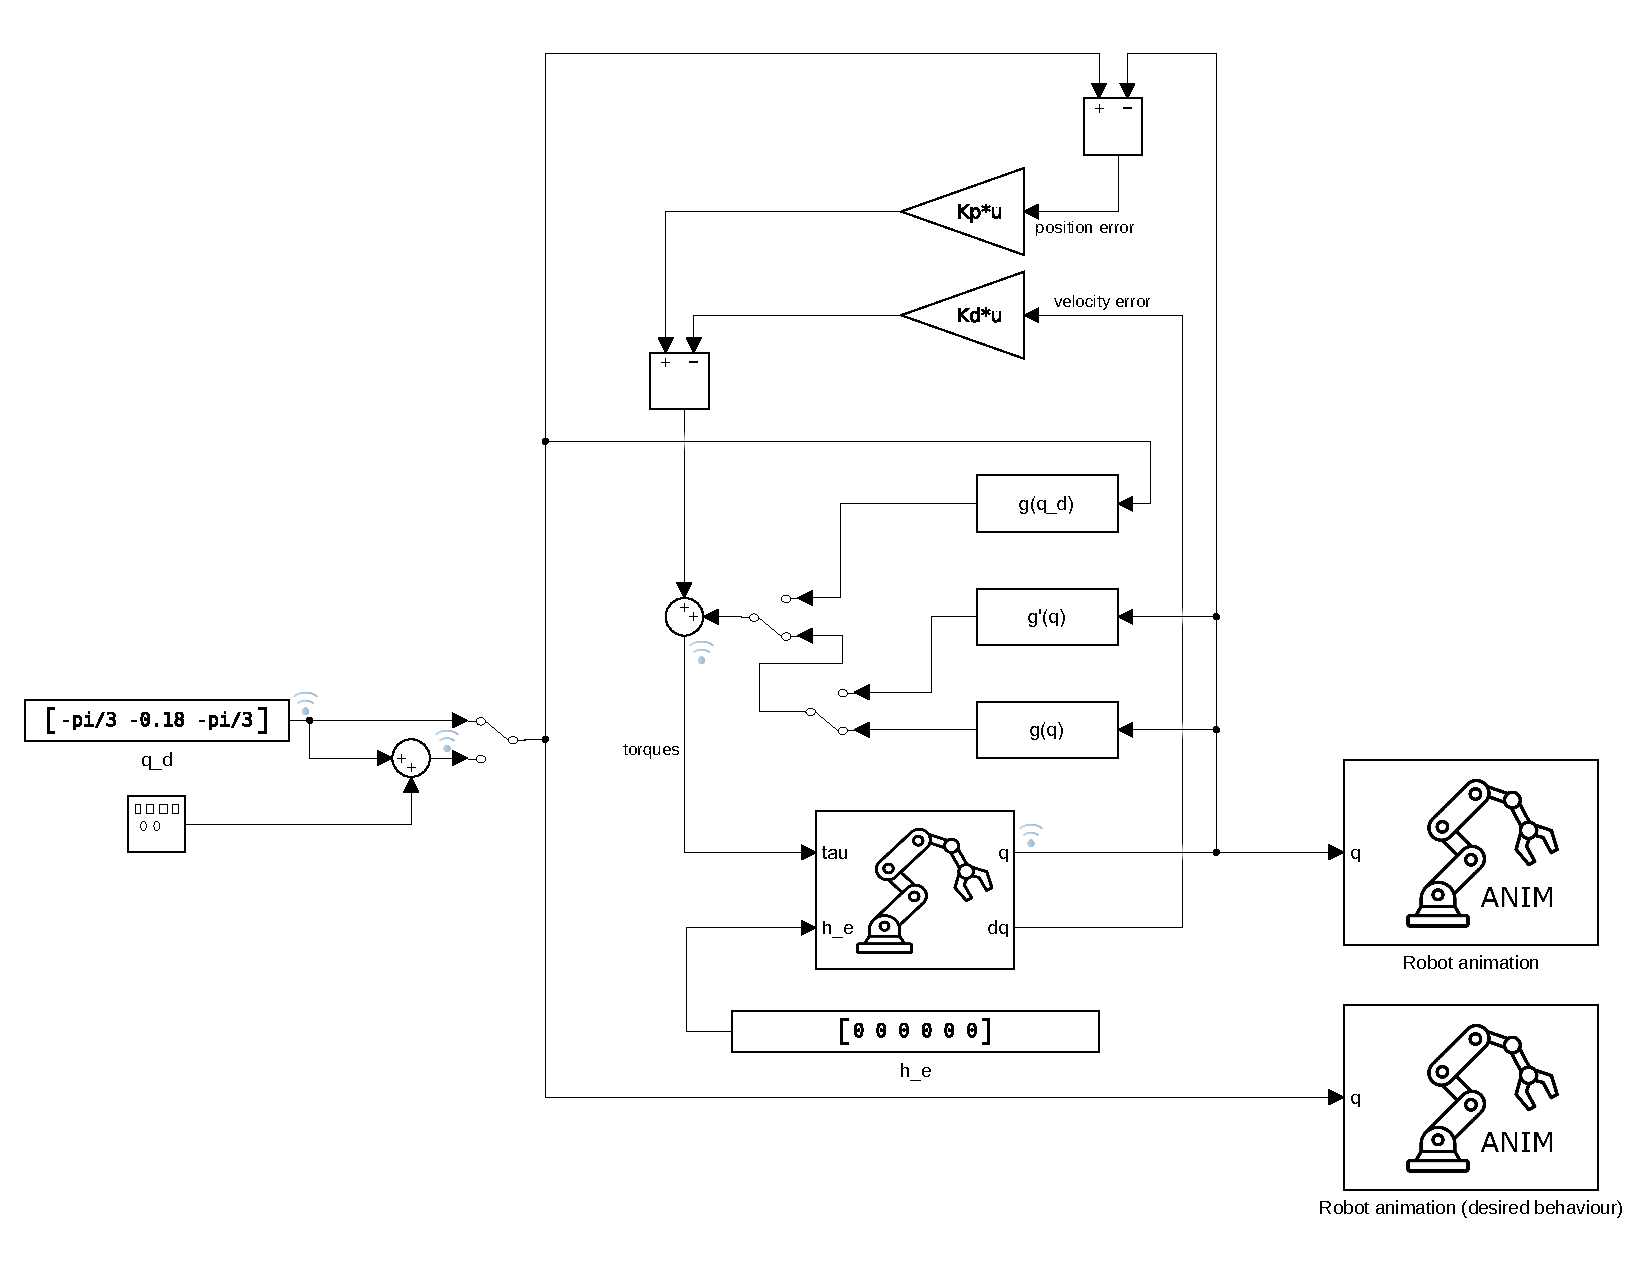
\includegraphics[scale=0.7]{schemes/joint_space_PD_with_gravity_comp/PD_with_g_compensation_scheme.pdf}
    }

    \caption{Joint Space PD control law with gravity compensation control scheme}
    \label{fig:js_PD_gravity_compensation_scheme}
\end{figure}

\begin{figure}[H]
    \noindent
    \makebox[\textwidth]{
        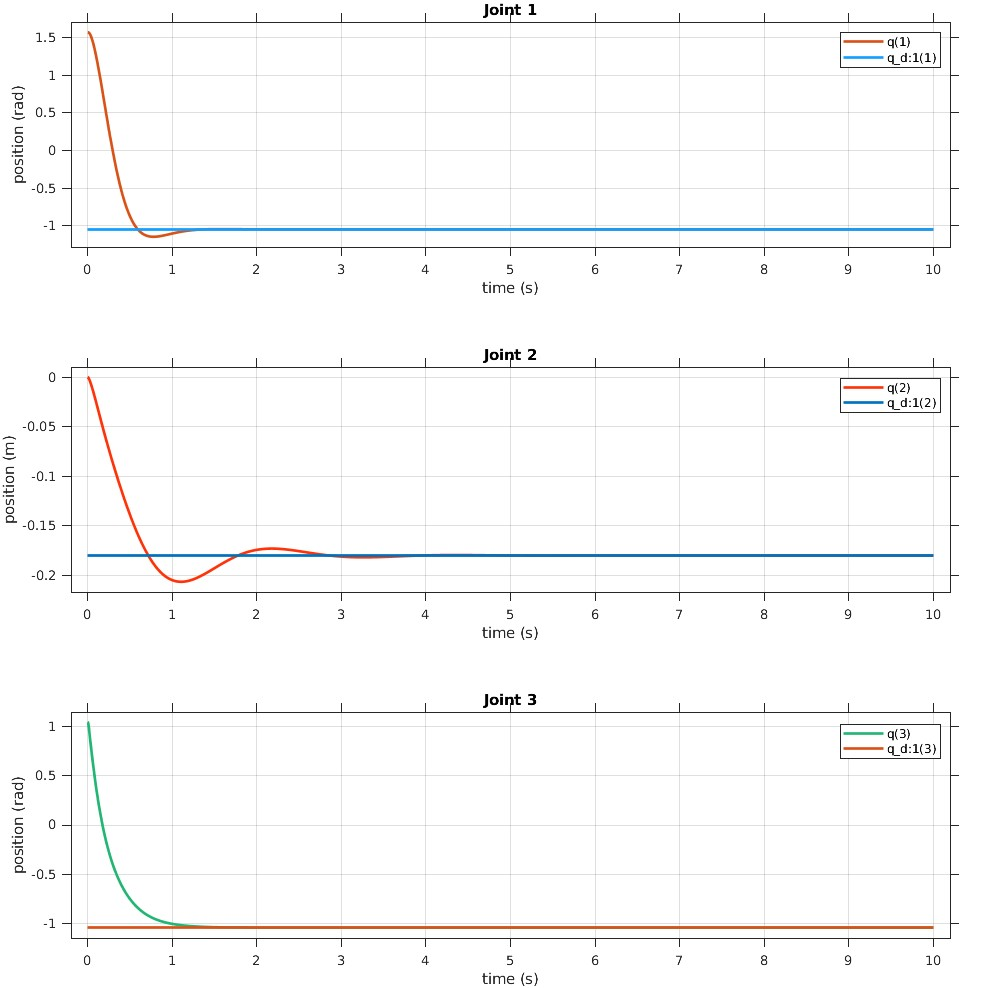
\includegraphics[scale=0.5]{schemes/joint_space_PD_with_gravity_comp/joints.jpg}
    }

    \caption{Joint Space PD control law with gravity compensation}
    \label{fig:js_PD_gravity_compensation_joints}
\end{figure}

\begin{figure}[H]
    \captionsetup{justification=centering}
    \noindent
    \makebox[\textwidth]{
        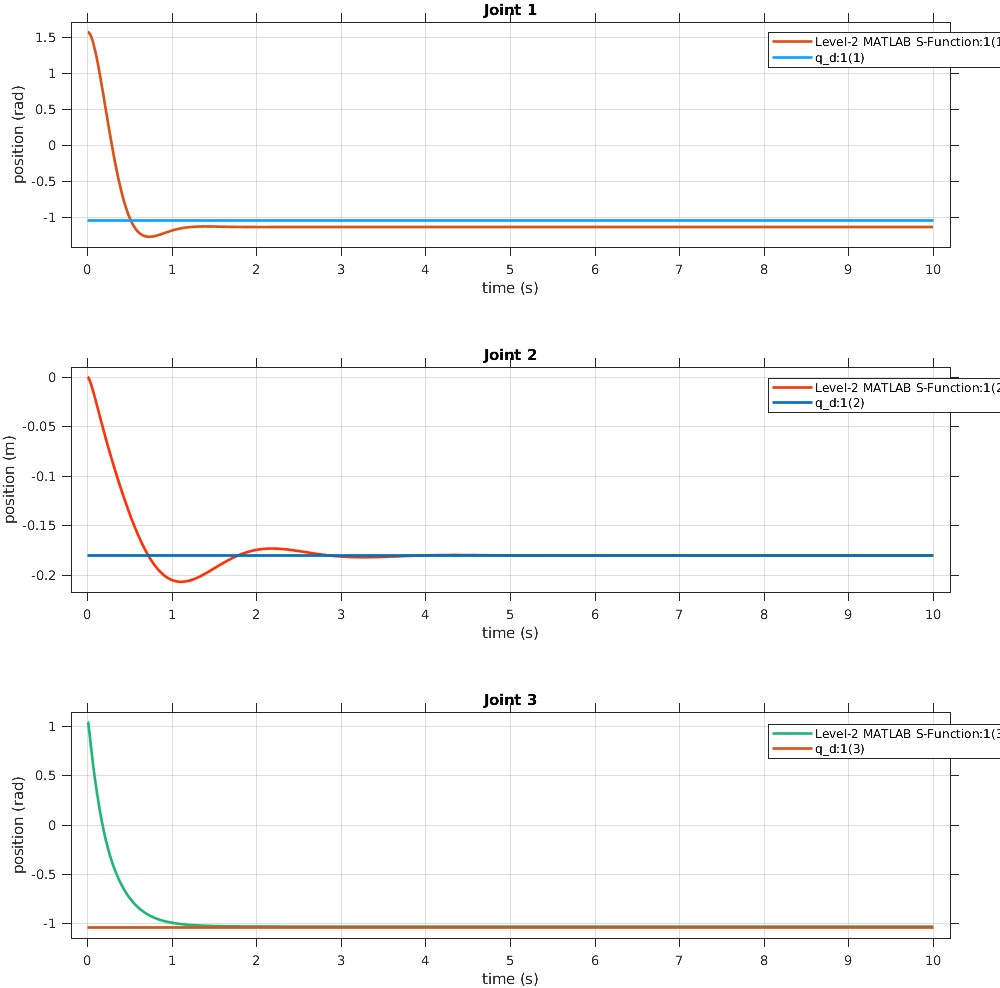
\includegraphics[scale=0.5]{schemes/joint_space_PD_with_gravity_comp/joints_wrong_g.jpg}
    }

    \caption{Joint Space PD control law with gravity compensation \\ compensated gravity term is $g'(q)$}
    \label{fig:js_PD_gravity_compensation_joint_wrong_g}
\end{figure}

\begin{figure}[H]
    \captionsetup{justification=centering}
    \noindent
    \makebox[\textwidth]{
        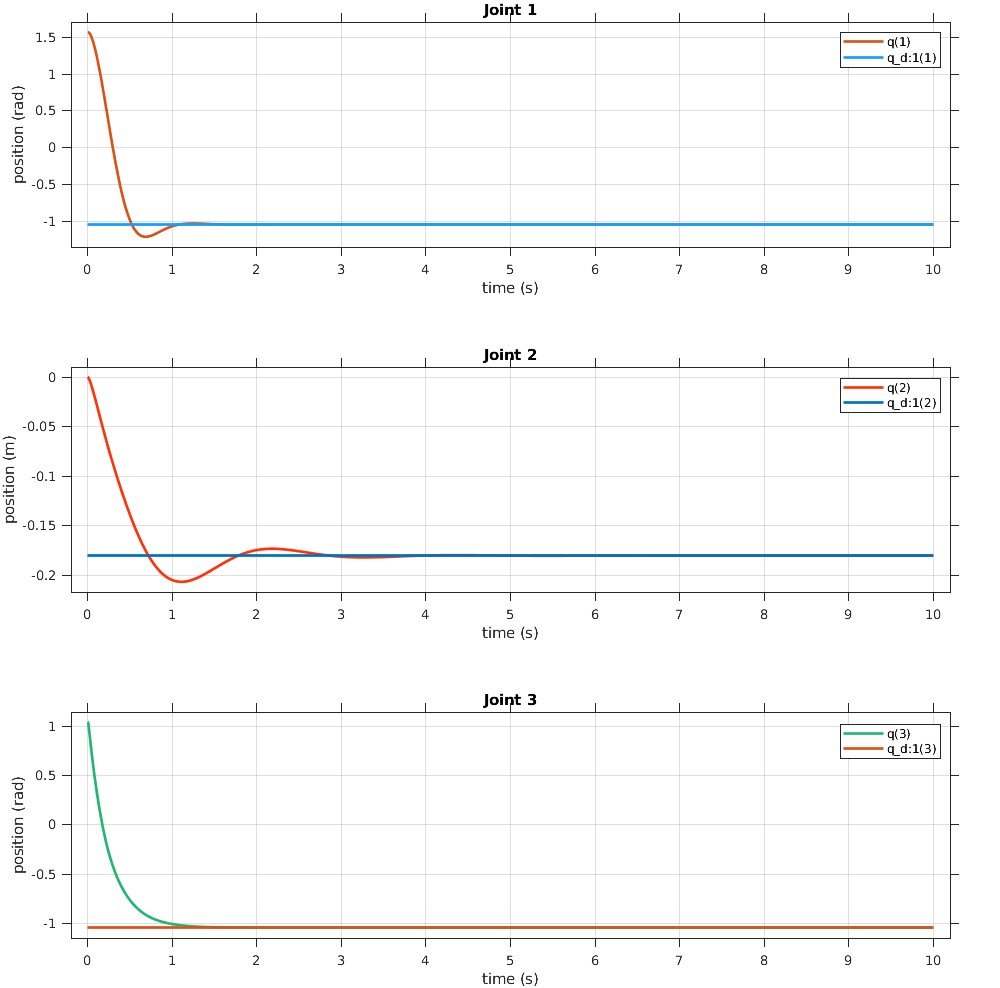
\includegraphics[scale=0.5]{schemes/joint_space_PD_with_gravity_comp/joints_g_of_q_d.jpg}
    }

    \caption{Joint Space PD control law with gravity compensation \\ compensated gravity term is $g(q_d)$}
    \label{fig:js_PD_gravity_compensation_joint_wrong_g}
\end{figure}




\begin{figure}[H]
    \captionsetup{justification=centering}
    \noindent
    \makebox[\textwidth]{
        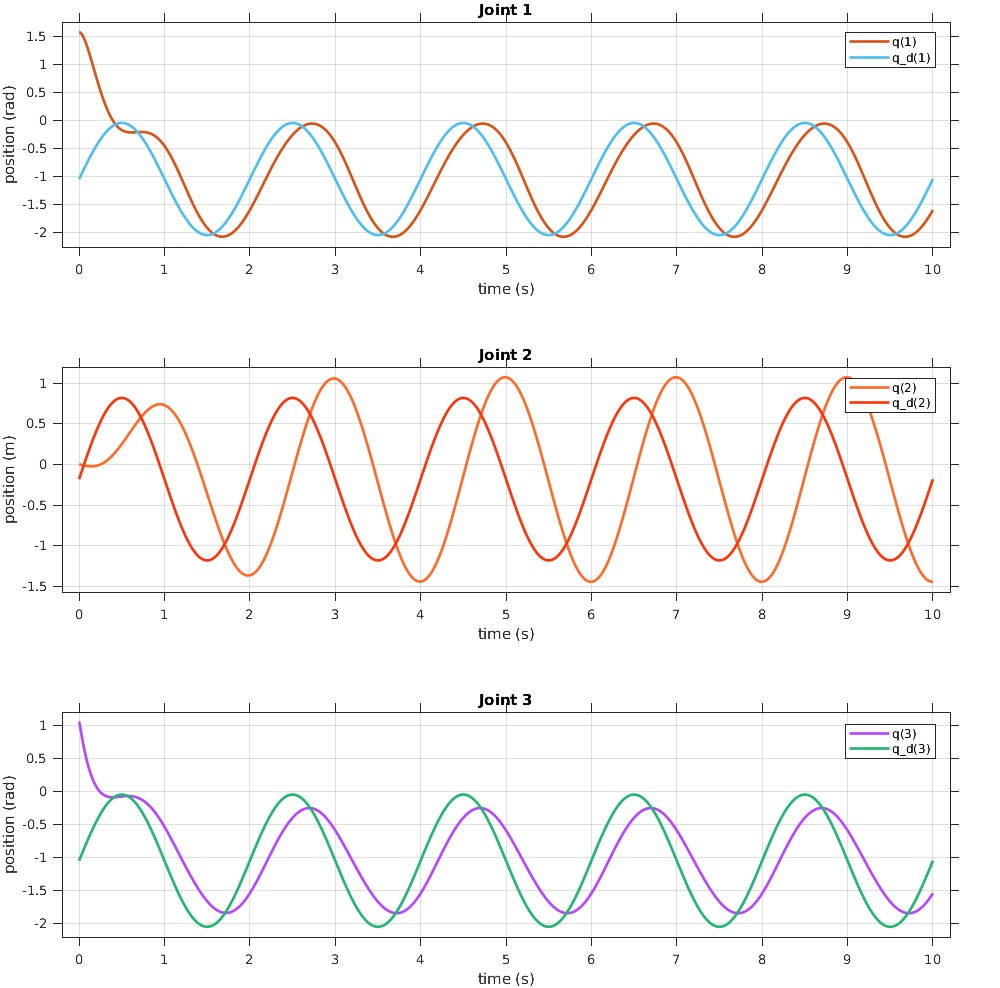
\includegraphics[scale=0.5]{schemes/joint_space_PD_with_gravity_comp/joints_tracking.jpg}
    }

    \caption{Joint Space PD control law with gravity compensation \\ tracking task}
    \label{fig:js_PD_gravity_compensation_tracking}
\end{figure}

\subsection{Joint Space Inverse Dynamics control law}

\begin{figure}[H]
    \noindent
    \makebox[\textwidth]{
        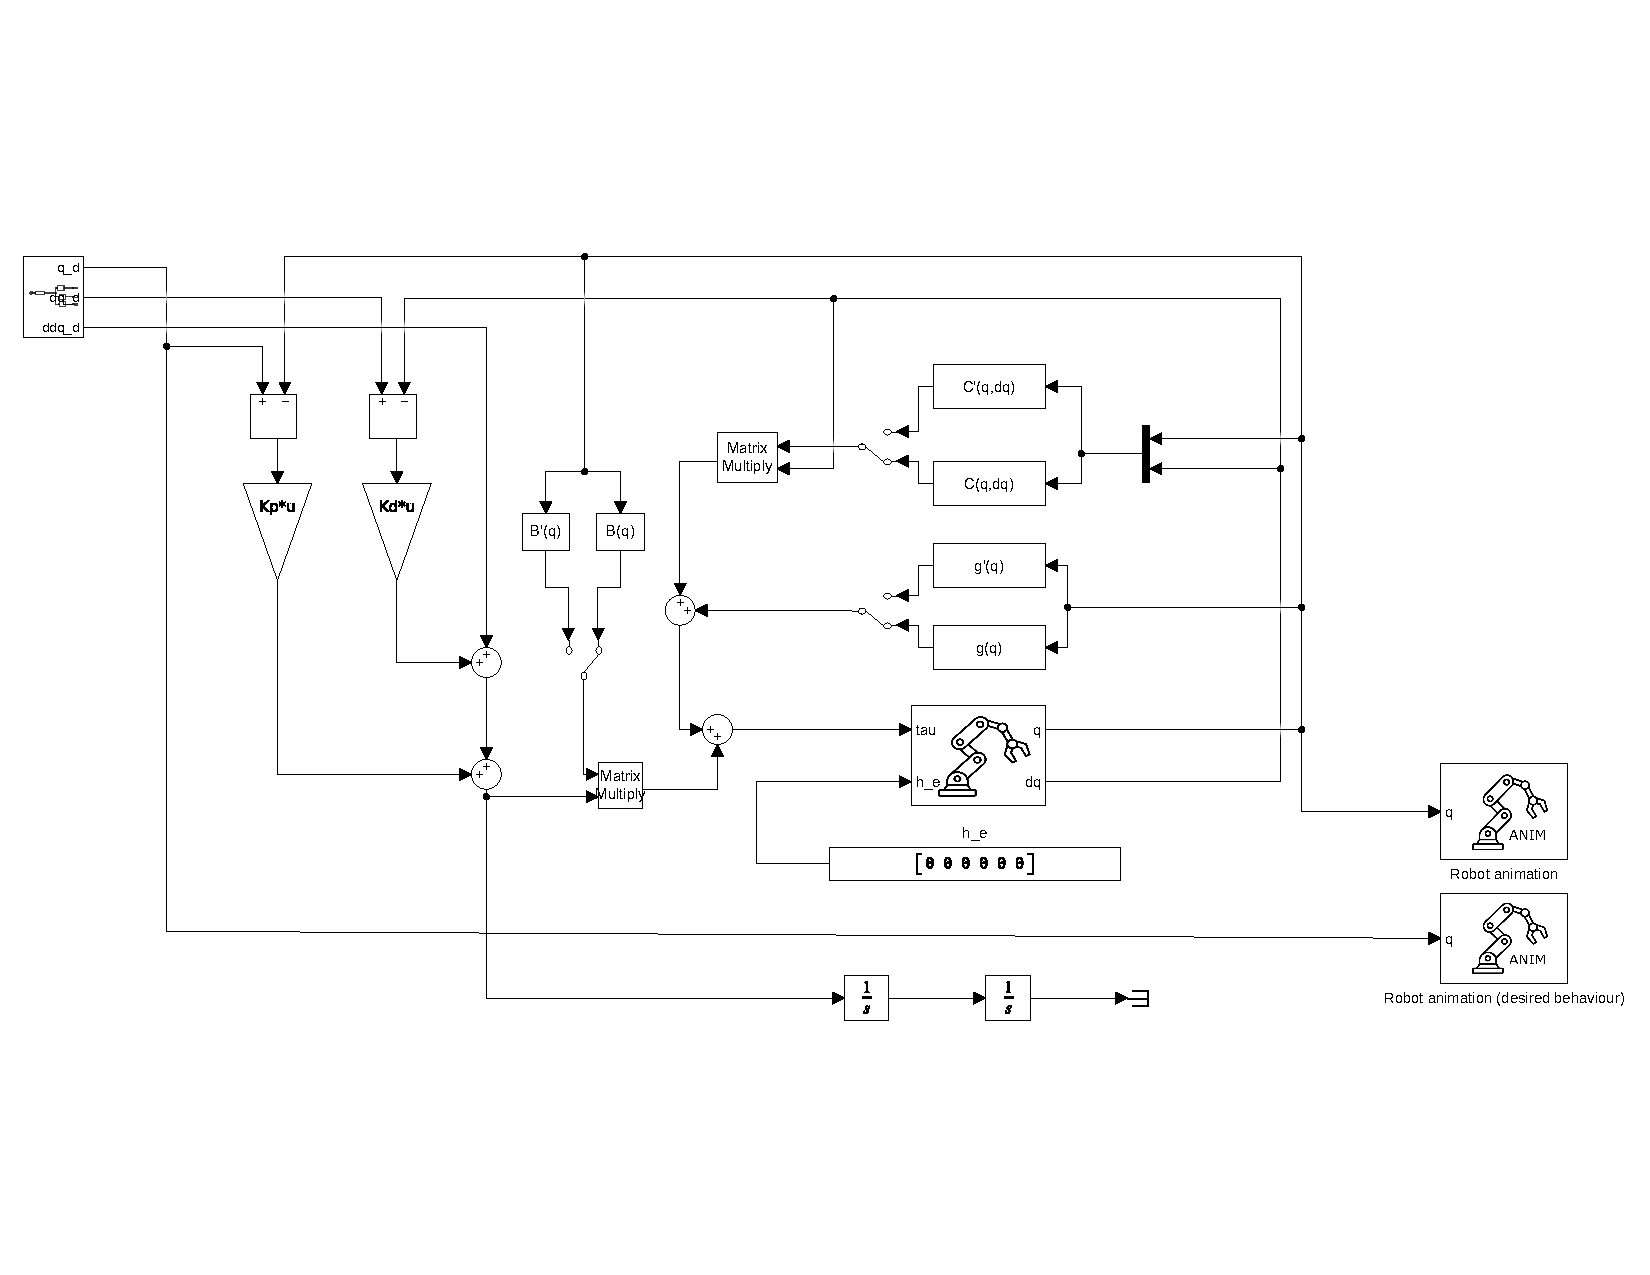
\includegraphics[scale=0.7]{schemes/joint_space_inverse_dynamics/Inverse_dynamics_control.pdf}
    }

    \caption{Joint Space Inverse Dynamics control law control scheme}
    \label{fig:js_Inverse_dynamics_scheme}
\end{figure}


\begin{figure}[H]
    \noindent
    \makebox[\textwidth]{
        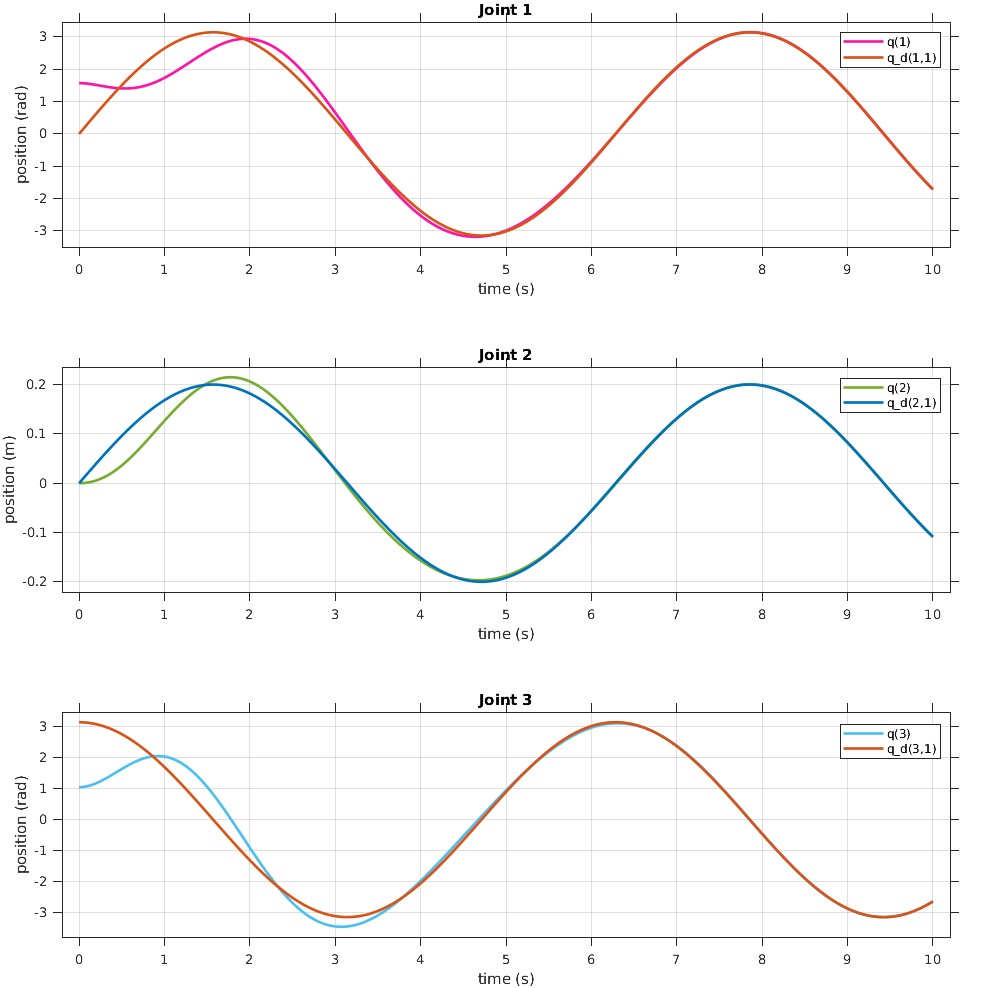
\includegraphics[scale=0.5]{schemes/joint_space_inverse_dynamics/joints.jpg}
    }

    \caption{Joint Space Inverse Dynamics control law}
    \label{fig:js_Inverse_dynamics_joints}
\end{figure}

\begin{figure}[H]
    \noindent
    \makebox[\textwidth]{
        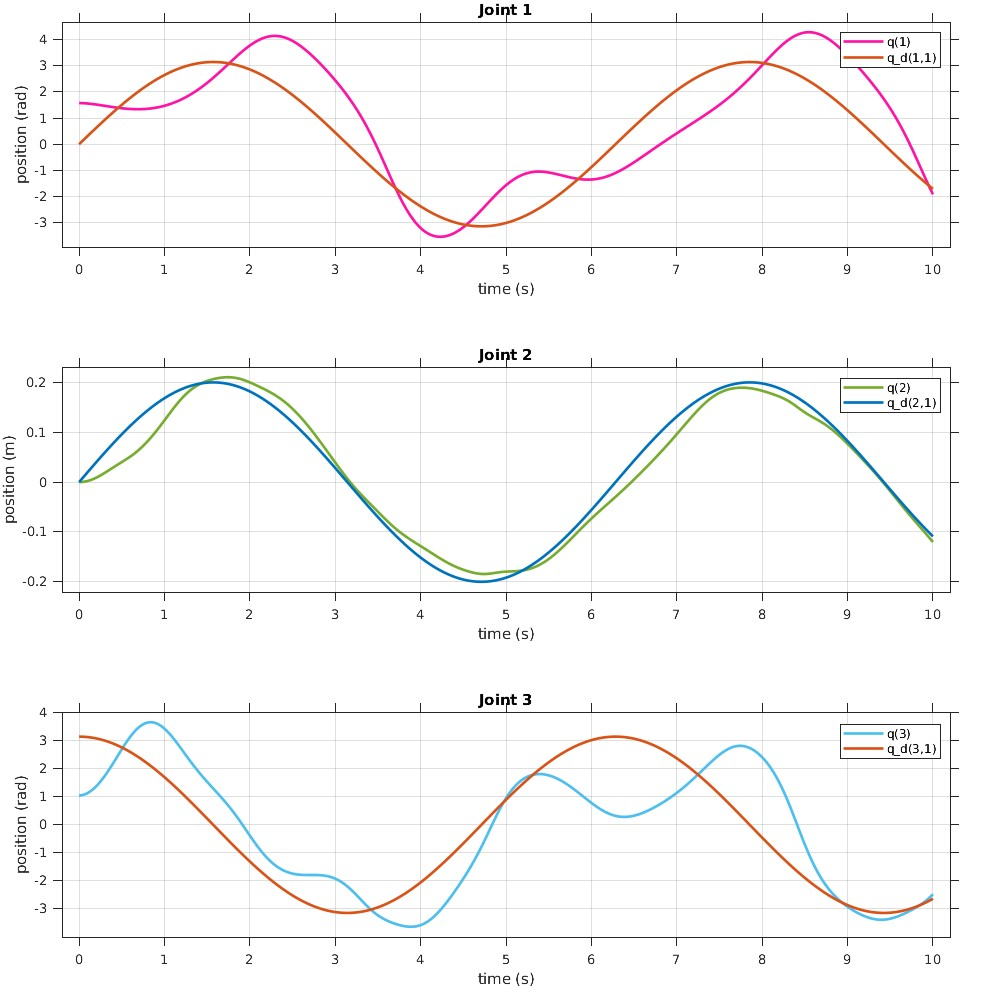
\includegraphics[scale=0.5]{schemes/joint_space_inverse_dynamics/joints_wrong_dynamics_matrices.jpg}
    }

    \caption{Joint Space Inverse Dynamics control law \\ dynamics matrices are off}
    \label{fig:js_Inverse_dynamics_joits_wrong_dynamics}
\end{figure}


\subsection{Operations Space PD control law with gravity compensation}


\begin{figure}[H]
    \noindent
    \makebox[\textwidth]{
        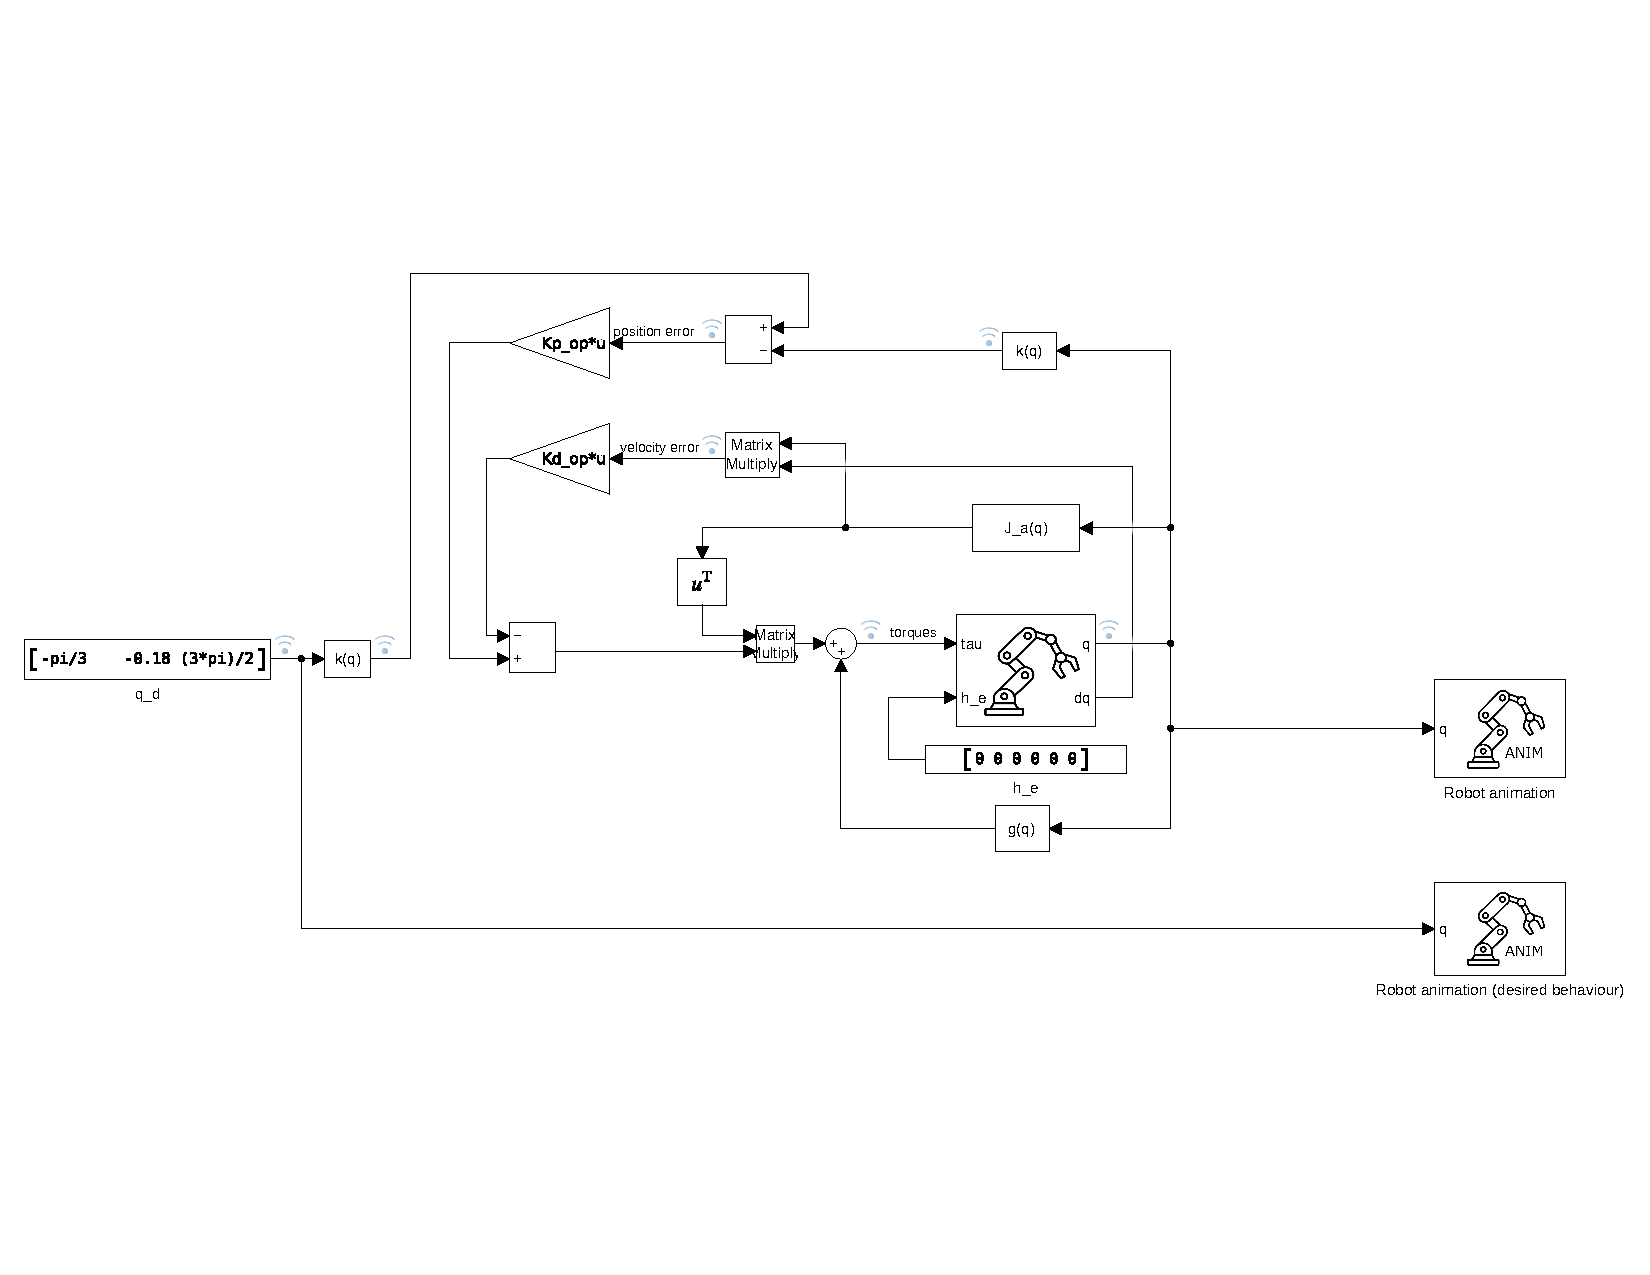
\includegraphics[scale=0.7]{schemes/op_space_PD_with_gravity_comp/PD_with_g_compensation_op_space_scheme.pdf}
    }

    \caption{Operational Space PD control law with gravity compensation scheme}
    \label{fig:op_space_PD_g_comp_scheme}
\end{figure}

\begin{figure}[H]
    \noindent
    \makebox[\textwidth]{
        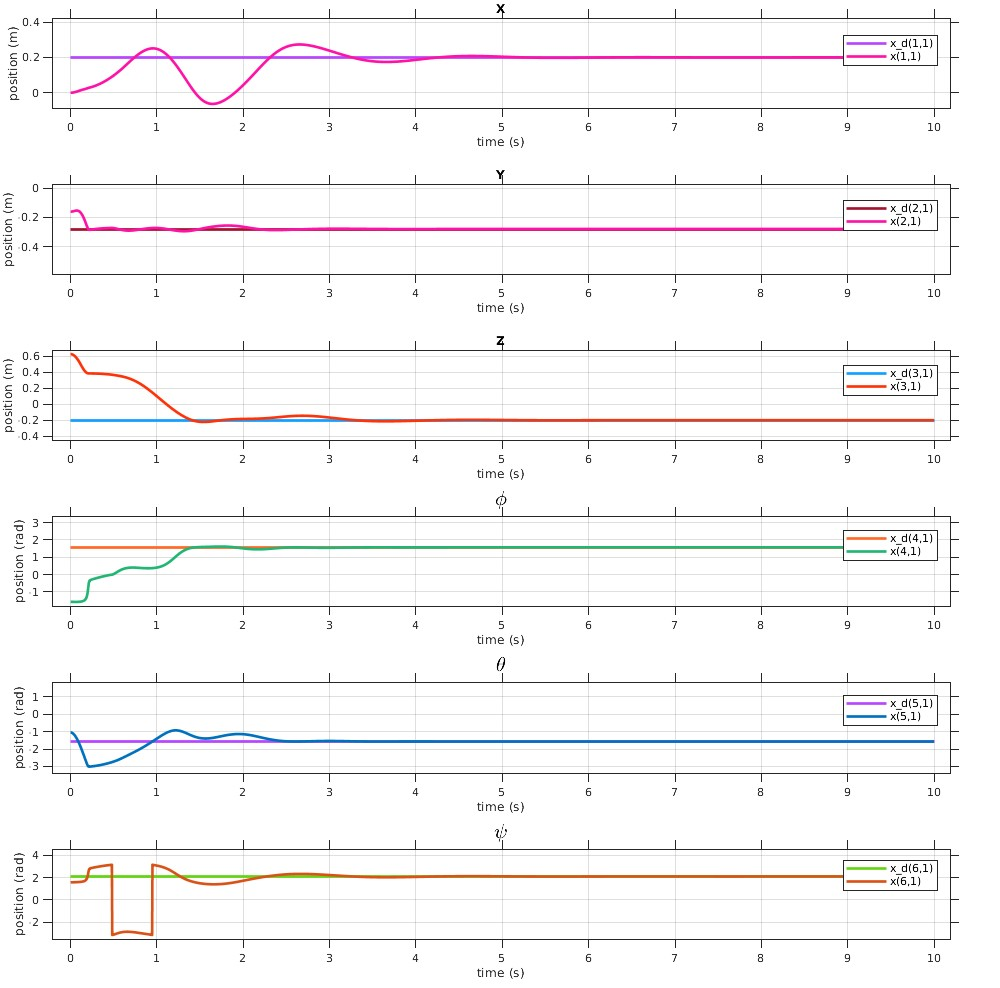
\includegraphics[scale=0.5]{schemes/op_space_PD_with_gravity_comp/joints.jpg}
    }

    \caption{Operational Space PD control law with gravity compensation}
    \label{fig:op_space_PD_g_comp_joints}
\end{figure}



\end{document}
